% CVPR Paper Template; see https://github.com/cvpr-org/author-kit

\documentclass[10pt,twocolumn,letterpaper]{article}

%%%%%%%%% PAPER TYPE
\usepackage[pagenumbers]{cvpr} % Clean version with page numbers (no review line numbers)

% Import additional packages in the preamble file, before hyperref
%% This file contains a number of tweaks that are typically applied to the main document.
%% They are not enabled by default, but can be enabled by uncommenting the relevant lines.


%%
%% Official support for 2-column teaser figure
%%
\usepackage{cuted} %< for strip environment

%%
%% For auto-referencing of figures (see fig/teaser.tex and \label{} therein) 
%%
\usepackage{currfile} %< for \currfilebase macro

%%
%% caption and (global) spacing overrides
%%
\usepackage{caption} %< for "\captionof" commands (teaser)
% \setlength{\abovecaptionskip}{.5em} % space above caption
% \setlength{\belowcaptionskip}{1em} % space below caption

%%
%% Inline annotations; for predefined colors, refer to "dvipsnames" in the xcolor package:
%% https://tinyurl.com/overleaf-colors
%%
\newcommand{\red}[1]{{\color{red}#1}}
\newcommand{\todo}[1]{{\color{red}#1}}
\newcommand{\TODO}[1]{\textbf{\color{red}[TODO: #1]}}
%%
%% Disable for camera ready / submission by uncommenting these lines:
%%
% \renewcommand{\TODO}[1]{}
% \renewcommand{\todo}[1]{#1}

%%
%% Work harder in optimizing text layout. Typically shrinks text by 1/6 of page, enable
%% it at the very end of the writing process, when you are just above the page limit.
%%
\usepackage{microtype}
\usepackage{listings}
\definecolor{codebg}{rgb}{0.97,0.97,0.98}
\definecolor{codeborder}{rgb}{0.85,0.87,0.90}
\definecolor{codekw}{rgb}{0.00,0.35,0.70}
\definecolor{codestr}{rgb}{0.64,0.08,0.08}
\definecolor{codecomm}{rgb}{0.38,0.44,0.48}
\lstset{
  language=Python,
  backgroundcolor=\color{codebg},
  basicstyle=\ttfamily\scriptsize,
  keywordstyle=\color{codekw}\bfseries,
  stringstyle=\color{codestr},
  commentstyle=\color{codecomm}\itshape,
  morekeywords={self,torch,F,True,False,None},
  frame=single,
  rulecolor=\color{codeborder},
  framerule=0.5pt,
  framesep=3pt,
  breaklines=true,
  columns=fullflexible,
  keepspaces=true,
  showstringspaces=false,
  aboveskip=5pt,
  belowskip=5pt,
  xleftmargin=3pt,
  xrightmargin=3pt
}

%%
%% Fine-tune paragraph spacing.
%%
% \renewcommand{\paragraph}[1]{\vspace{.5em}\noindent\textbf{#1.}}

%%
%% Globally adjusts space between figure and caption.
%%
% \setlength{\abovecaptionskip}{.5em}

%%
%% Allows "the use of \paper to refer to the project name"
%% with automatic management of space at the end of the word.
%%
% \usepackage{xspace}
% \newcommand{\paper}{ProjectName\xspace}

%%
%% Commonly used math definitions.
%%
% \DeclareMathOperator*{\argmin}{arg\,min}
% \DeclareMathOperator*{\argmax}{arg\,max}

%%
%% Tighten underline.
%%
% \usepackage{soul}
% \setuldepth{foobar}

%%
%% Reconfigure paragraph (tweaks spacing)
%%


\definecolor{cvprblue}{rgb}{0.21,0.49,0.74}
\usepackage[pagebackref,breaklinks,colorlinks,allcolors=cvprblue]{hyperref}

\def\confName{02516}
\def\confYear{2025}


\title{Image Segmentation on PH2 and DRIVE: Architectures, Metrics, and Loss Ablations}


\author{
\parbox{0.8\textwidth}{\centering
Kal Adam Kalo (s246525), Author Name (s246526), Author Name (s246527),
Author Name (s246528), Author Name (s246529)
}
}


\begin{document}
\maketitle

% ============================================================================
% MAIN REPORT BODY (Strictly <= 3 pages including all tables and figures)
% ============================================================================
\begin{abstract}
We investigate binary semantic segmentation under both full and weak supervision across PH2 (skin lesions) and DRIVE (retinal blood vessels). In Part~1, we compare an encoder-decoder CNN and a U-Net across five metrics and ablate BCE, Focal, and positive-weighted BCE losses. In Part~2, we train U-Net on PH2 using only sparse point clicks with a partial BCE loss, finding that just $25+25$ clicks ($<0.08\%$ of pixels) match full supervision ($0.8808$ vs.\ $0.8796$ Test Dice), and compare uniform vs.\ interior-biased click sampling.
\end{abstract}

\section{Datasets and Splits}
\label{sec:datasets}

We evaluate our segmentation models on two medical imaging datasets located at \texttt{/dtu/datasets1/02516}:

\begin{itemize}
    \item \textbf{PH2 (Skin Lesion Segmentation):} Contains 200 RGB dermoscopic images (\texttt{.bmp}) with resolutions around $767 \times 576$ pixels (ranging from $761\text{--}769 \times 572\text{--}577$) and corresponding binary lesion masks (\texttt{*\_lesion.bmp}). Because PH2 has no pre-assigned splits, we shuffle the 200 cases with a fixed seed (\texttt{seed=42}) and split them 70\% / 15\% / 15\% into \textbf{140 training}, \textbf{30 validation}, and \textbf{30 test} images. Images are resized to $256 \times 256$ using bilinear interpolation, and masks using nearest-neighbor interpolation to preserve binary labels.
    \item \textbf{DRIVE (Retinal Blood Vessel Segmentation):} Contains 40 RGB fundus images (\texttt{.tif}, $565 \times 584$ pixels) pre-split into \texttt{training/} (20 images) and \texttt{test/} (20 images). Crucially, DRIVE provides two mask types: manual retinal vessel segmentations in \texttt{training/1st\_manual/} (\texttt{*\_manual1.gif}) and field-of-view (FOV) masks in \texttt{training/mask/} and \texttt{test/mask/} (\texttt{*\_mask.gif}). Because \texttt{test/} lacks vessel ground-truth masks, we use only the 20 labeled images from \texttt{training/} (with \texttt{1st\_manual/} vessel masks) and split them 70\% / 15\% / 15\% (\texttt{seed=42}) into \textbf{14 training}, \textbf{3 validation}, and \textbf{3 test} images, resized to $512 \times 512$ (bilinear for images, nearest-neighbor for masks).
\end{itemize}

\section{Methods and Evaluation Metrics}
\label{sec:methods}

\subsection{Evaluation Metrics}
We evaluate all models using five pixel-wise metrics computed from true positives (TP), false positives (FP), true negatives (TN), and false negatives (FN):
\begin{itemize}
    \item \textbf{Dice:} $\frac{2\text{TP}}{2\text{TP}+\text{FP}+\text{FN}}$ \quad \textbf{IoU:} $\frac{\text{TP}}{\text{TP}+\text{FP}+\text{FN}}$
    \item \textbf{Accuracy:} $\frac{\text{TP}+\text{TN}}{\text{TP}+\text{TN}+\text{FP}+\text{FN}}$ \quad \textbf{Sensitivity:} $\frac{\text{TP}}{\text{TP}+\text{FN}}$ \quad \textbf{Specificity:} $\frac{\text{TN}}{\text{TN}+\text{FP}}$
\end{itemize}
\textbf{Strengths and Weaknesses:} Accuracy and Specificity include TN and are therefore dominated by background pixels under class imbalance. On DRIVE, where vessels occupy $<10\%$ of pixels, predicting all background already yields $\text{Accuracy} = 0.9164$ and $\text{Specificity} = 1.0000$ while $\text{Dice} = 0$. Sensitivity measures foreground recall (crucial for thin retinal vessels) but ignores FP; conversely, Dice and IoU ignore TN and directly measure foreground overlap, with IoU penalizing errors more strongly ($\text{IoU} \le \text{Dice}$). On PH2, lesions are larger ($\sim 35\%$ foreground), making Accuracy more informative, though Dice/IoU remain preferable for boundary quality.

\subsection{Network Architectures}
\textbf{EncDec Baseline:} A 4-stage encoder-decoder CNN with 64-channel $3\times3$ convolutions, $2\times2$ max-pooling, a $64$-channel bottleneck, and nearest-neighbor $2\times$ upsampling (no skip connections).

\textbf{U-Net:} A 4-level U-Net (\texttt{base\_channels=32}) using double $3\times3$ Conv-BN-ReLU blocks, $2\times2$ max-pooling, transposed-convolution $2\times$ upsampling, and channel-wise skip connections (\texttt{torch.cat}). Using $256\times256$ (PH2) and $512\times512$ (DRIVE) preserves fine vessel detail while keeping all feature maps divisible by $16$:
\begin{center}
\small
\begin{tabular}{@{}lcc@{}}
\toprule
Layer & PH2 ($256\times256$) & DRIVE ($512\times512$) \\
\midrule
\texttt{enc1 / dec1} & $32\times256\times256$ & $32\times512\times512$ \\
\texttt{enc2 / dec2} & $64\times128\times128$ & $64\times256\times256$ \\
\texttt{enc3 / dec3} & $128\times64\times64$  & $128\times128\times128$ \\
\texttt{enc4 / dec4} & $256\times32\times32$  & $256\times64\times64$ \\
\texttt{bottleneck}  & $512\times16\times16$  & $512\times32\times32$ \\
\texttt{output}      & $1\times256\times256$  & $1\times512\times512$ \\
\bottomrule
\end{tabular}
\end{center}
\begin{lstlisting}[caption={U-Net decoder skip concatenation (\texttt{UNetModel.py}).}]
u4 = self.up4(b)
d4 = self.dec4(torch.cat([u4, e4], dim=1)) # + up3..up1
out = self.head(d1)
\end{lstlisting}

\subsection{Loss Functions and Weak Supervision}
To address class imbalance, we compare three pixel-wise losses on raw logits $\hat{y}$: (1) standard \textbf{Binary Cross-Entropy (BCE)}; (2) \textbf{Focal Loss}~\cite{lin2017focal} ($\gamma=2.0$), which scales BCE by $(1-p_t)^\gamma$ to focus gradients on hard pixels; and (3) \textbf{Positive-Weighted BCE}, scaling positive errors by $w_{\text{pos}}$ ($2.0$ on PH2, $8.0$ on DRIVE).

For Part~2 (weak supervision on PH2), we replace full training masks with simulated positive/negative point clicks while keeping the \texttt{U-Net}, splits ($140/30/30$), and hyperparameters ($256\times256$, $50$ epochs, Adam $\text{lr}=10^{-3}$) identical. We train with a \textbf{Partial Point BCE} loss evaluated only over the binary click mask $M \in \{0,1\}^{H\times W}$:
$\mathcal{L}_{\text{pt}} = \frac{\sum_{i} M_i \,\ell_{\text{BCE}}(\hat{y}_i, y_i)}{\max(\sum_{i} M_i, 1)}$.
We compare \textbf{Uniform} sampling (random foreground/background pixels) against \textbf{Interior} sampling ($11\times11$ mask erosion for positive clicks and $15\times15$ dilation exclusion for negative clicks) to mimic human annotators clicking away from ambiguous borders.
\begin{lstlisting}[caption={Focal, Partial Point BCE (\texttt{losses.py}), and Interior click sampling (\texttt{PH2WeakDataset.py}).}]
# FocalLoss.forward
bce = F.binary_cross_entropy_with_logits(y_pred, y_true, reduction="none")
pt = torch.sigmoid(y_pred) * y_true + (1 - torch.sigmoid(y_pred)) * (1 - y_true)
loss = ((1.0 - pt).pow(self.gamma) * bce).mean()

# PointBCELoss.forward
bce = F.binary_cross_entropy_with_logits(y_pred, click_target, reduction="none")
loss = (bce * click_mask).sum() / click_mask.sum().clamp(min=1.0)

# Interior click regions (PH2WeakDataset)
pos_region = _erode_mask(m, kernel_size=11)
neg_region = ~_dilate_mask(m, kernel_size=15)
\end{lstlisting}

\section{Experiments and Discussion}
\label{sec:results}

\begin{table}[t]
\centering
\caption{Part~1: \texttt{EncDec} vs.\ \texttt{U-Net} (BCE) on PH2 ($256\times256$) and DRIVE ($512\times512$).}
\label{tab:main_results}
\scriptsize
\begin{tabular}{@{}lllccccc@{}}
\toprule
Dataset & Model & Split & Dice & IoU & Acc & Sens & Spec \\
\midrule
PH2 & EncDec & Train & 0.9439 & 0.8937 & 0.9627 & 0.9682 & 0.9601 \\
PH2 & EncDec & Val   & 0.9302 & 0.8696 & 0.9497 & 0.9495 & 0.9498 \\
PH2 & EncDec & Test  & 0.8750 & 0.7777 & 0.9269 & 0.8919 & 0.9410 \\
\midrule
PH2 & U-Net  & Train & 0.9373 & 0.8819 & 0.9593 & 0.9395 & 0.9688 \\
PH2 & U-Net  & Val   & 0.9371 & 0.8816 & 0.9559 & 0.9287 & 0.9708 \\
PH2 & U-Net  & Test  & \textbf{0.8796} & \textbf{0.7851} & \textbf{0.9316} & 0.8715 & \textbf{0.9558} \\
\midrule
DRIVE & EncDec & Train & 0.4065 & 0.2551 & 0.9198 & 0.3199 & 0.9761 \\
DRIVE & EncDec & Val   & 0.4407 & 0.2826 & 0.9192 & 0.3808 & 0.9683 \\
DRIVE & EncDec & Test  & 0.4222 & 0.2676 & 0.9185 & 0.3266 & 0.9779 \\
\midrule
DRIVE & U-Net  & Train & 0.8198 & 0.6946 & 0.9698 & 0.8002 & 0.9857 \\
DRIVE & U-Net  & Val   & 0.7997 & 0.6662 & 0.9669 & 0.7910 & 0.9829 \\
DRIVE & U-Net  & Test  & \textbf{0.7993} & \textbf{0.6658} & \textbf{0.9653} & \textbf{0.7577} & \textbf{0.9862} \\
\bottomrule
\end{tabular}
\end{table}

\subsection{Architecture & Loss Ablations (Part 1)}
As shown in Table~\ref{tab:main_results}, \texttt{EncDec} performs well on PH2 ($\text{Test Dice}=0.8750$) due to large lesions, while \texttt{U-Net} reaches $0.8796$. On DRIVE, \texttt{EncDec} fails to capture thin vessels ($\text{Test Dice}=0.4222$, $\text{Sens}=0.3266$), whereas \texttt{U-Net} skip connections nearly double Test Dice to $0.7993$ ($\text{Sens}=0.7577$).

In Table~\ref{tab:loss_ablation}, Focal Loss ($\gamma=2$) achieves the best PH2 Test Dice ($0.8823$) by emphasizing hard boundaries. On DRIVE, Weighted BCE ($w=8$) boosts vessel Sensitivity ($0.7577 \to 0.8276$) but lowers Specificity ($0.9862 \to 0.9721$) and Dice ($0.7993 \to 0.7860$) due to thicker boundary false positives.

\begin{table}[t]
\centering
\caption{Part~1: Loss ablation on \texttt{U-Net} (Test split).}
\label{tab:loss_ablation}
\scriptsize
\begin{tabular}{@{}llccccc@{}}
\toprule
Dataset & Loss & Dice & IoU & Acc & Sens & Spec \\
\midrule
PH2 & BCE                 & 0.8796 & 0.7851 & 0.9316 & 0.8715 & \textbf{0.9558} \\
PH2 & Focal ($\gamma=2$)  & \textbf{0.8823} & \textbf{0.7894} & \textbf{0.9324} & 0.8844 & 0.9516 \\
PH2 & Weighted BCE ($w=2$)& 0.8789 & 0.7840 & 0.9288 & \textbf{0.9011} & 0.9399 \\
\midrule
DRIVE & BCE                 & \textbf{0.7993} & \textbf{0.6658} & \textbf{0.9653} & 0.7577 & \textbf{0.9862} \\
DRIVE & Focal ($\gamma=2$)  & 0.7963 & 0.6616 & 0.9645 & 0.7604 & 0.9850 \\
DRIVE & Weighted BCE ($w=8$)& 0.7860 & 0.6475 & 0.9589 & \textbf{0.8276} & 0.9721 \\
\bottomrule
\end{tabular}
\end{table}

\subsection{Weak Point Supervision on PH2 (Part 2)}
Table~\ref{tab:weak_results} shows that \texttt{U-Net} trained with only $1+1$ clicks already reaches $0.7202$ Test Dice, rising steadily with $5+5$ ($0.8345$) and $10+10$ ($0.8592$). At $25+25$ clicks ($50$ pixels/image, $<0.08\%$ of $256^2$), weak supervision reaches $0.8808$ Test Dice, matching full supervision ($0.8796$) before saturating at $50+50$ ($0.8769$). Comparing sampling strategies at $10+10$ clicks, \texttt{Interior} slightly improves Val Dice ($0.9068$ vs.\ $0.9031$) and Test Specificity ($0.9665$ vs.\ $0.9567$) but lowers Sensitivity ($0.8058$ vs.\ $0.8342$) because avoiding boundary clicks removes border supervision, causing slight under-segmentation.

\begin{table}[t]
\centering
\caption{Part~2: Weak point-click supervision on PH2 (\texttt{U-Net}, Test split) vs.\ full supervision ($65{,}536$ px/img).}
\label{tab:weak_results}
\scriptsize
\begin{tabular}{@{}llccccc@{}}
\toprule
Clicks (pos+neg) & Strategy & Dice & IoU & Acc & Sens & Spec \\
\midrule
1 + 1   & Uniform  & 0.7202 & 0.5627 & 0.8407 & 0.7148 & 0.8914 \\
5 + 5   & Uniform  & 0.8345 & 0.7160 & 0.9040 & 0.8444 & 0.9279 \\
10 + 10 & Uniform  & 0.8592 & 0.7531 & 0.9216 & 0.8342 & 0.9567 \\
10 + 10 & Interior & 0.8531 & 0.7438 & 0.9204 & 0.8058 & \textbf{0.9665} \\
25 + 25 & Uniform  & \textbf{0.8808} & \textbf{0.7870} & 0.9301 & \textbf{0.9003} & 0.9422 \\
50 + 50 & Uniform  & 0.8769 & 0.7807 & 0.9310 & 0.8568 & 0.9608 \\
\midrule
Full Mask & Full   & 0.8796 & 0.7851 & \textbf{0.9316} & 0.8715 & 0.9558 \\
\bottomrule
\end{tabular}
\end{table}

\begin{figure*}[t]
\centering
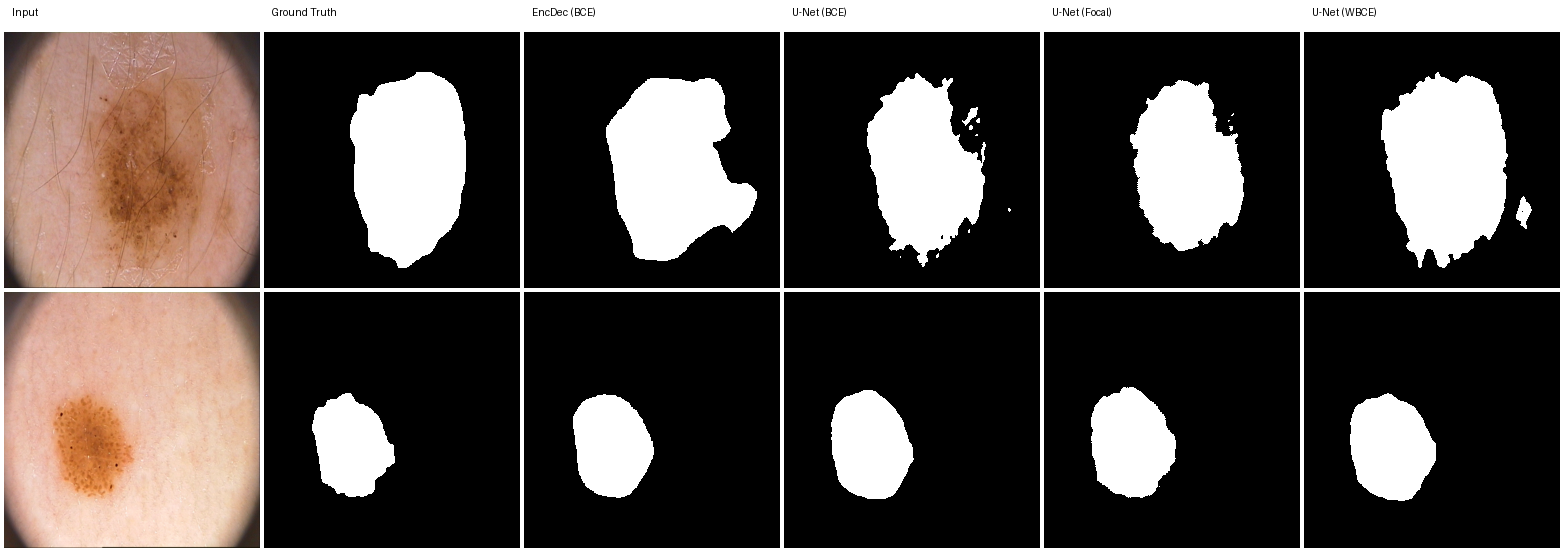
\includegraphics[width=0.95\textwidth]{fig/qualitative_ph2.png}\\[3pt]
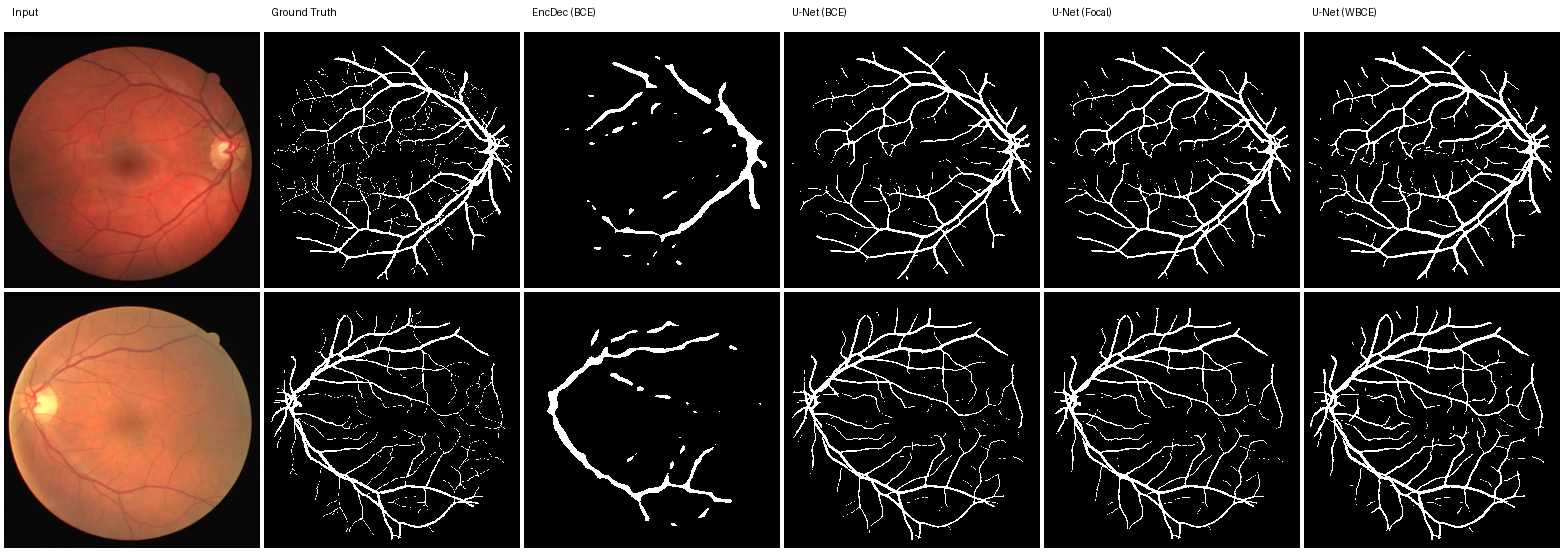
\includegraphics[width=0.95\textwidth]{fig/qualitative_drive.png}
\caption{Qualitative test-set predictions on PH2 (top two rows) and DRIVE (bottom two rows). \texttt{U-Net} recovers fine retinal vessel structures missed by \texttt{EncDec}, while Weighted BCE increases vessel sensitivity at the expense of thicker boundary predictions.}
\label{fig:qualitative}
\end{figure*}


% ============================================================================
% REFERENCES & GENERATIVE AI STATEMENT (Excluded from the 3-page limit)
% ============================================================================
\clearpage
{
    \small
    \bibliographystyle{ieeenat_fullname}
    \bibliography{main}
}
\section*{Statement on the Use of Generative AI}
We used Google Antigravity (AI coding assistant) as an engineering and writing aid across Parts~1 and~2. Specifically, it was used to:
\begin{itemize}
    \item Simulate point-click weak supervision (\texttt{PH2WeakDataset}).
    \item Debug starter code issues (missing imports, hardcoded \texttt{nn.Upsample} dimensions in \texttt{EncDec}, and \texttt{BCELoss} variable typos).
    \item Troubleshoot DTU HPC environment setup (virtual environment creation and PyTorch CUDA compatibility for Tesla V100).
    \item Structure and format the 3-page CVPR \LaTeX\ report.
\end{itemize}


\end{document}
